\documentclass[12pt,a4paper,oneside]{article}
\usepackage{amsmath,amsthm}
\usepackage{graphicx}
\usepackage{ctex}
\usepackage{float}
\usepackage{subfigure}
\usepackage{caption}

\title{计算方法编程作业一实验报告}
\author{张博厚 PB22071354}
\date{}

\begin{document}
\maketitle
\tableofcontents

\section{实验内容}
本实验要求编程求解一反射问题的二维简化模型: 将镜面假定为圆形, 给定观察点P与物点Q, 
输出反射点T和像点R.

\section{算法}
\subsection{计算反射点T}
对于反射点T,参考《Computational Mirror Cup and Saucer Art》中的方法,使用二分法数值求解:
假定观察点P在x轴负半轴,物点Q在第二象限, P与Q均在圆外, G为过点P在第二象限内所作切线的
切点, 如图1所示.
\begin{figure}[htbp]
    \centering
    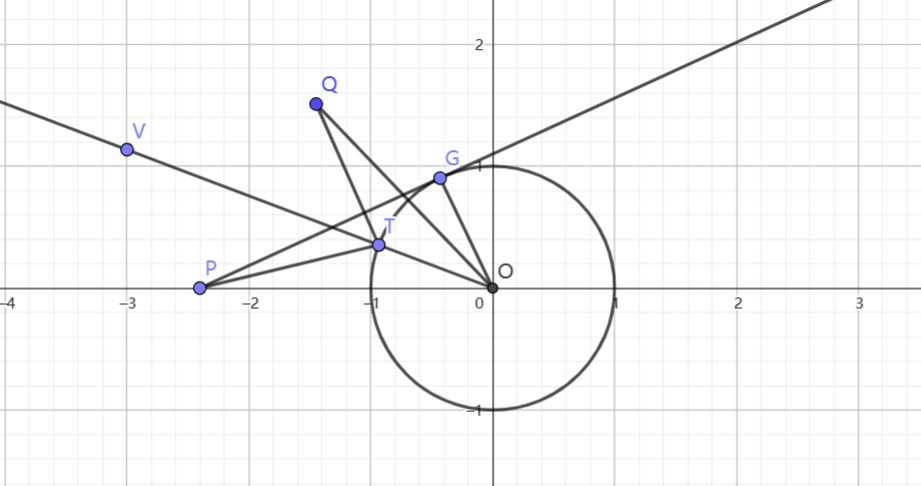
\includegraphics[width = 0.77\textwidth]{figs/f.png}
    \caption{反射模型及各点示意图}
\end{figure}\par
通过二分法确定$\angle POT$的大小,进而确定T的位置, 首先应分别计算$\angle POG, \angle POQ$
的大小:
$$\angle POG = \arccos{\dfrac{1}{\lvert x_P \rvert}}$$
$$  \angle POQ = \arccos{\dfrac{\lvert x_Q \rvert}{\sqrt{x_Q^2+y_Q^2}}}$$
用二分的方式,取初值$high=min\{\angle POG,\angle POQ\},\ low=0$,每次令
$\angle POT = \frac{1}{2}(low+high)$, 可知T的坐标为$(-\cos{\angle POT}, \sin{\angle POT})$.下面
分别计算$\angle PTV, \angle QTV$: 由T坐标可得直线OT方程:
\begin{equation}
    \sin{\angle POT}\ x+\cos{\angle POT}\ y=0
\end{equation}
故P,Q两点到直线OT的距离分别为
\begin{equation*}
    l_1 = \dfrac{\lvert \sin{\angle POT}\ x_P+\cos{\angle POT}\ y_P \rvert}{\sin{\angle POT}^2+\cos{\angle POT}^2 }
        =\lvert \sin{\angle POT}\ x_P+\cos{\angle POT}\ y_P \rvert
\end{equation*}
\begin{equation*}
    l_2 = \lvert \sin{\angle POT}\ x_Q+\cos{\angle POT}\ y_Q \rvert
\end{equation*}
于是
$$\angle PTV = \arcsin{\dfrac{l_1}{\lvert PT \rvert}}$$
$$\angle QTV = \arcsin{\dfrac{l_2}{\lvert QT \rvert}}$$
比较$\angle PTV$与$\angle QTV$的大小, 并据此调整二分的上限或下限, 直到两角误差在可接受的范围内
(实验中设置为double类型的精度15位), 此时的T即为所求反射点.

\subsection{计算像点R}
对于像点R, 在已知Q与T的前提下用解析法求解,实质上即为求解Q关于圆上过T切线的对称点.
(1)式写出直线OT方程, 由切线过T且与OT垂直, 可知切线方程为:
\begin{equation}
    l:\ y-y_T = -\dfrac{x_T}{y_T}(x-x_T)
\end{equation}
直线QR与直线l垂直, 因此QR的方程为:
\begin{equation}
    y-y_Q = \dfrac{y_T}{x_T}(x-x_Q)
\end{equation}
设直线QR与直线l的交点为M,联立(2)(3)式可得M坐标为:
\begin{equation}
    \begin{cases}
        x_M = x_Ty_T(y_T-y_Q)+x_T^3+y_T^2x_Q\\
        y_M = y_T-\dfrac{x_T}{y_T}(x_M-x_T)
    \end{cases}
\end{equation}
点Q与R关于切线l对称, 因而关于交点M中心对称, 由关系
\begin{equation}
    \begin{cases}
        x_R = 2x_M-x_Q\\
        y_R = 2y_M-y_Q
    \end{cases}
\end{equation}
即可求得像点R的坐标.

\section{实验结果}
对所给样例,计算结果如下:
\begin{figure}[H]
    \centering
    \subfigure{
        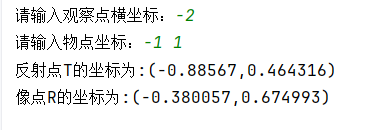
\includegraphics[scale = 0.75]{figs/r00.png}
    }
    \hspace{0.5in}
    \subfigure{
        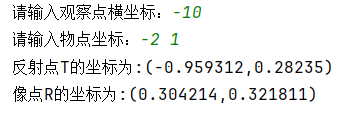
\includegraphics[scale = 0.75]{figs/r01.png}
    }
    \caption{所给样例}
\end{figure}\noindent
与参考数据相比,误差在允许范围内($10^{-6}$).\par
对自测数据,计算结果如下:
\begin{figure}[H]
    \centering
    \subfigure{
        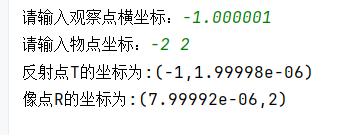
\includegraphics[scale = 0.75]{figs/r0.png}
    }
    \hspace{0.5in}
    \subfigure{
        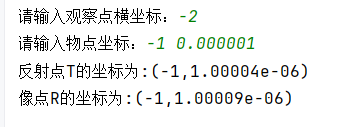
\includegraphics[scale = 0.75]{figs/r1.png}
    }
    \hspace{0.5in}
    \subfigure{
        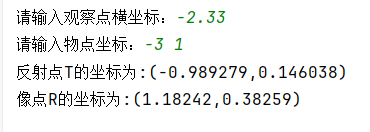
\includegraphics[scale = 0.7]{figs/r2.png}
    }
    \hspace{0.5in}
    \subfigure{
        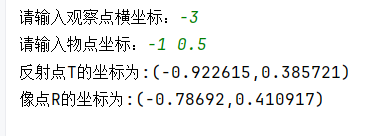
\includegraphics[scale = 0.7]{figs/r3.png}
    }
    \hspace{0.5in}
    \subfigure{
        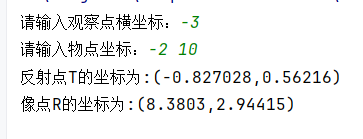
\includegraphics[scale = 0.7]{figs/r4.png}
    }
    \hspace{0.5in}
    \subfigure{
        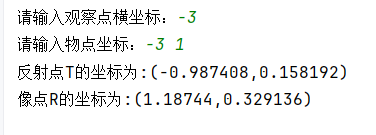
\includegraphics[scale = 0.7]{figs/r5.png}
    }
    \hspace{0.5in}
    \subfigure{
        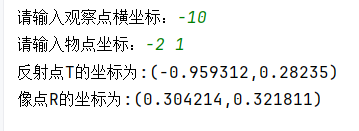
\includegraphics[scale = 0.75]{figs/r6.png}
    }
    \hspace{0.5in}
    \subfigure{
        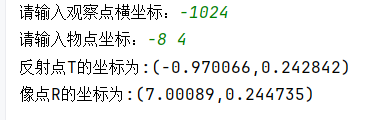
\includegraphics[scale = 0.75]{figs/r7.png}
    }
    \caption{自测数据}
\end{figure}

\section{分析与思考}\noindent
对比参考数据而言, 计算结果符合4位有效数字精度要求,但仍有一定误差存在, 主要原因如下:\\

\noindent1.double类型精度仅为15位, 进行多次计算后误差会逐次放大.\\
2.函数中调用了c++的cmath库, 进行了三角函数,反三角函数等计算,也会造成一定误差.\\
3.特别地, 在计算$\angle PTV, \angle QTV$时, 需要将$\lvert PT\rvert, \lvert QT \rvert$
作为分母, 因此当P与T,Q与T接近时(如自测数据1,2), 误差会比较大.
\end{document}